\subsection{Data description}
We have a two-class classification problem. The training data $Xtrain$ contains 1500 observations, each 32 dimensional. One training sample has 31 real valued features and 1 categorical feature, the 14th feature. Our task is to predict the category for unseen test data, consisting in 1500 samples. We measure the accuracy of our estimation using $RMSE$, $0-1 loss$ and $log-loss$. 

\subsection{Data visualization and cleaning}
We noticed the samples were not equally distributed among classes, about $35\%$ of the samples were coming from one class and $65\%$ from the other. We did not have time to study the implications of this on our model estimation. We changed the labeling from -1/1 to 0/1 because our cost function was better expressed using 0 and 1.

The training data was again not centered as seen in $Fig.$\ref{fig:dist_classification}
 After changing feature 14 to a dummy variable we normalized the data to have 0 mean and std 1.We noticed more outliers in the data of classification than in the one from regression. We removed outliers the same way as in the regression task which left us with 1431 samples (4$\%$ of the data).
{%%#figures/distribution_classification.png}
\begin{figure}[h]
  \begin{subfigure}[b]{0.5\textwidth}
   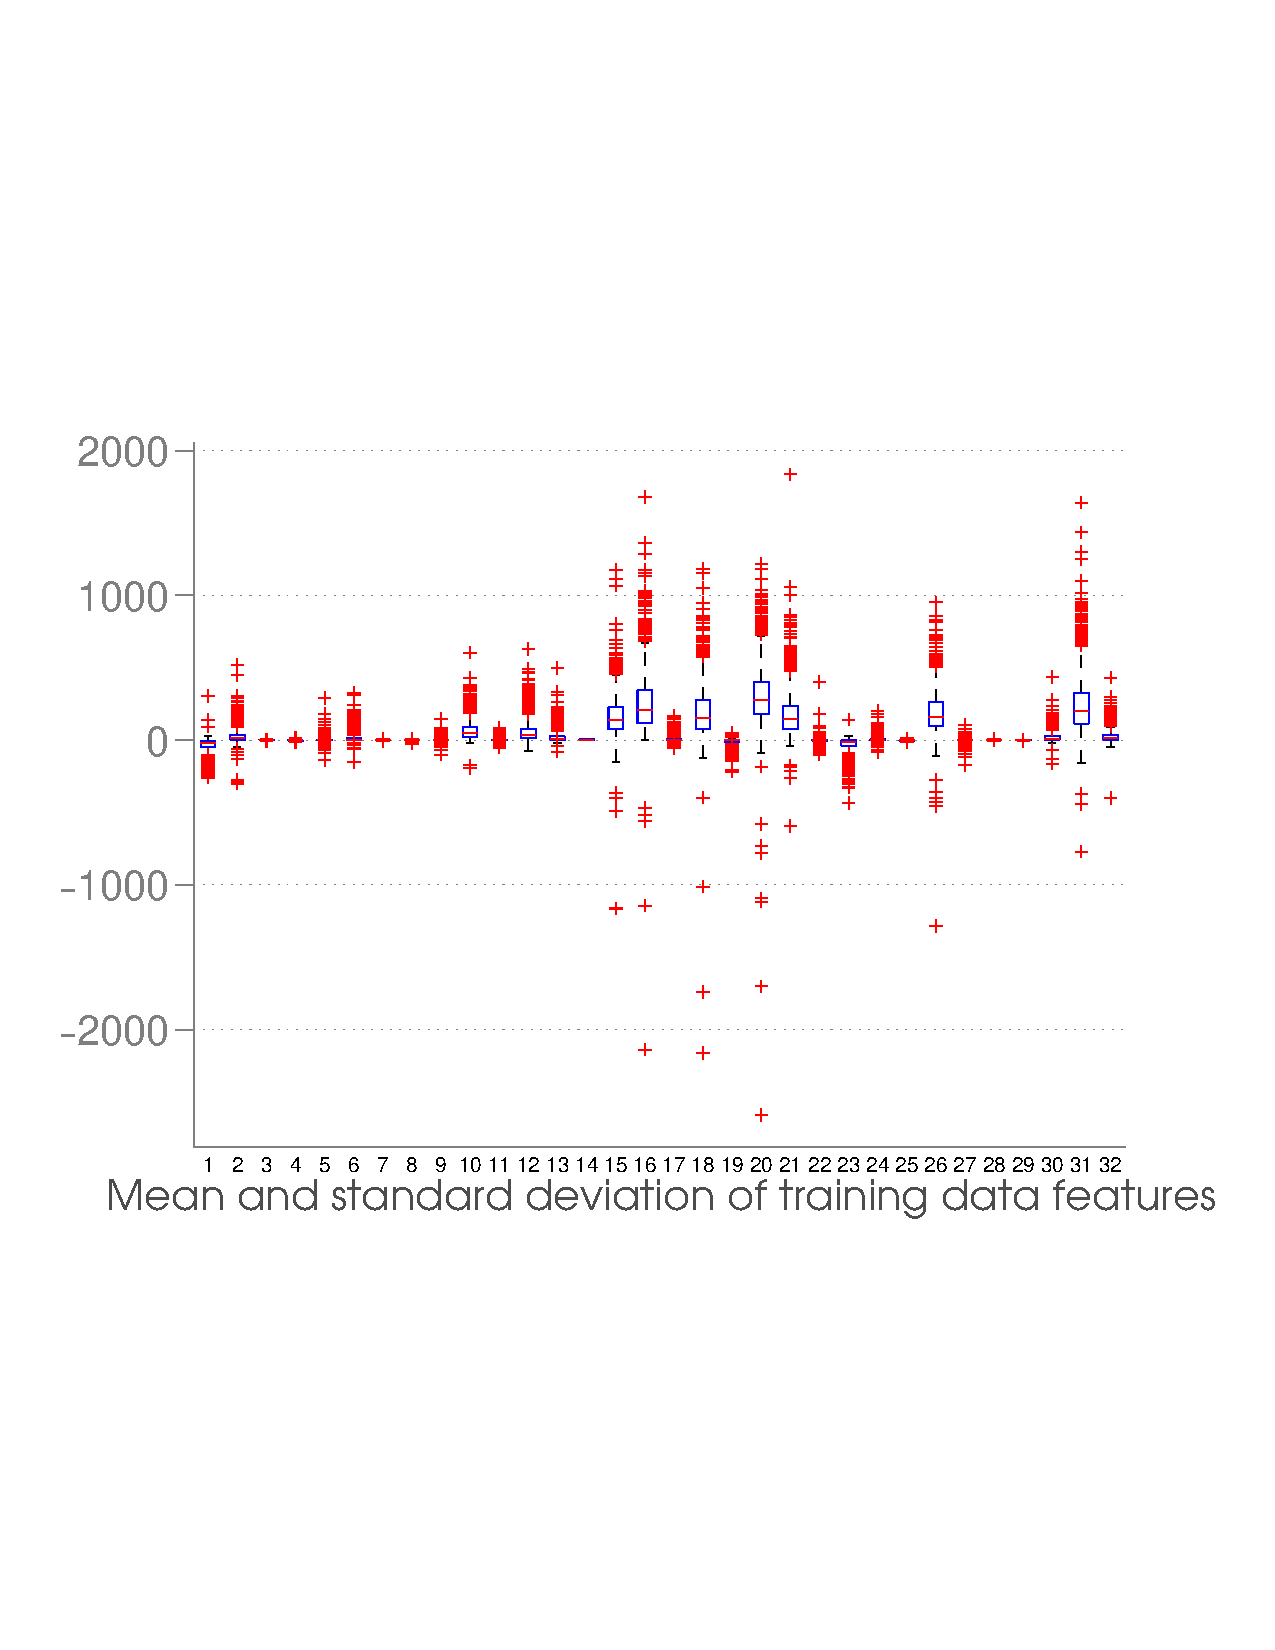
\includegraphics[width=\textwidth]{figures/classification_distribution.pdf}
    \caption{Mean and standard deviation for the training data features. The input is not normalised and contains outliers.}
    \label{fig:dist_classification}
  \end{subfigure}
  \caption{• Data visualization. }
\end{figure}

\subsection{Logistic Regression}

We applied Logistic regression and Penalized logistic Regression using gradient descent. Best results are obtained on the train accuracy of $97.14\%$ with value 10.0 for $\alpha$. We obtained the optimal $\alpha$ value for logistic regression classifier using cross validation technique where we split $50\%$ of the data for validation.

In penalized logistic regression, the choice of penalty factor ($\lambda$) is crucial. Therefore, we used cross validation procedure to estimate $\lambda$ when we divide $50\%$ of the data as test data and $50\%$ of the data as training data. The value of $\lambda$ varies from $10^{-2}$ to $10^3$ with 400 points in between. As can be seen in Figure \ref{fig:Lambda_pLr}, for smaller $\lambda$ values, training error is much lower than the test error while the test error gets as high as the training error  as the $\lambda$ increases which is a sign of under-fitting. 

For smaller $\lambda$ values, the training and test error estimated in penalized logistic regression shows very similar behavior in the training and test error estimated in logistic regression. The same $\alpha$ value that is obtained for the logistic regression method also gives the best accuracy for penalized logistic regression method.

\begin{figure}[h]
  \begin{subfigure}[b]{0.5\textwidth}
   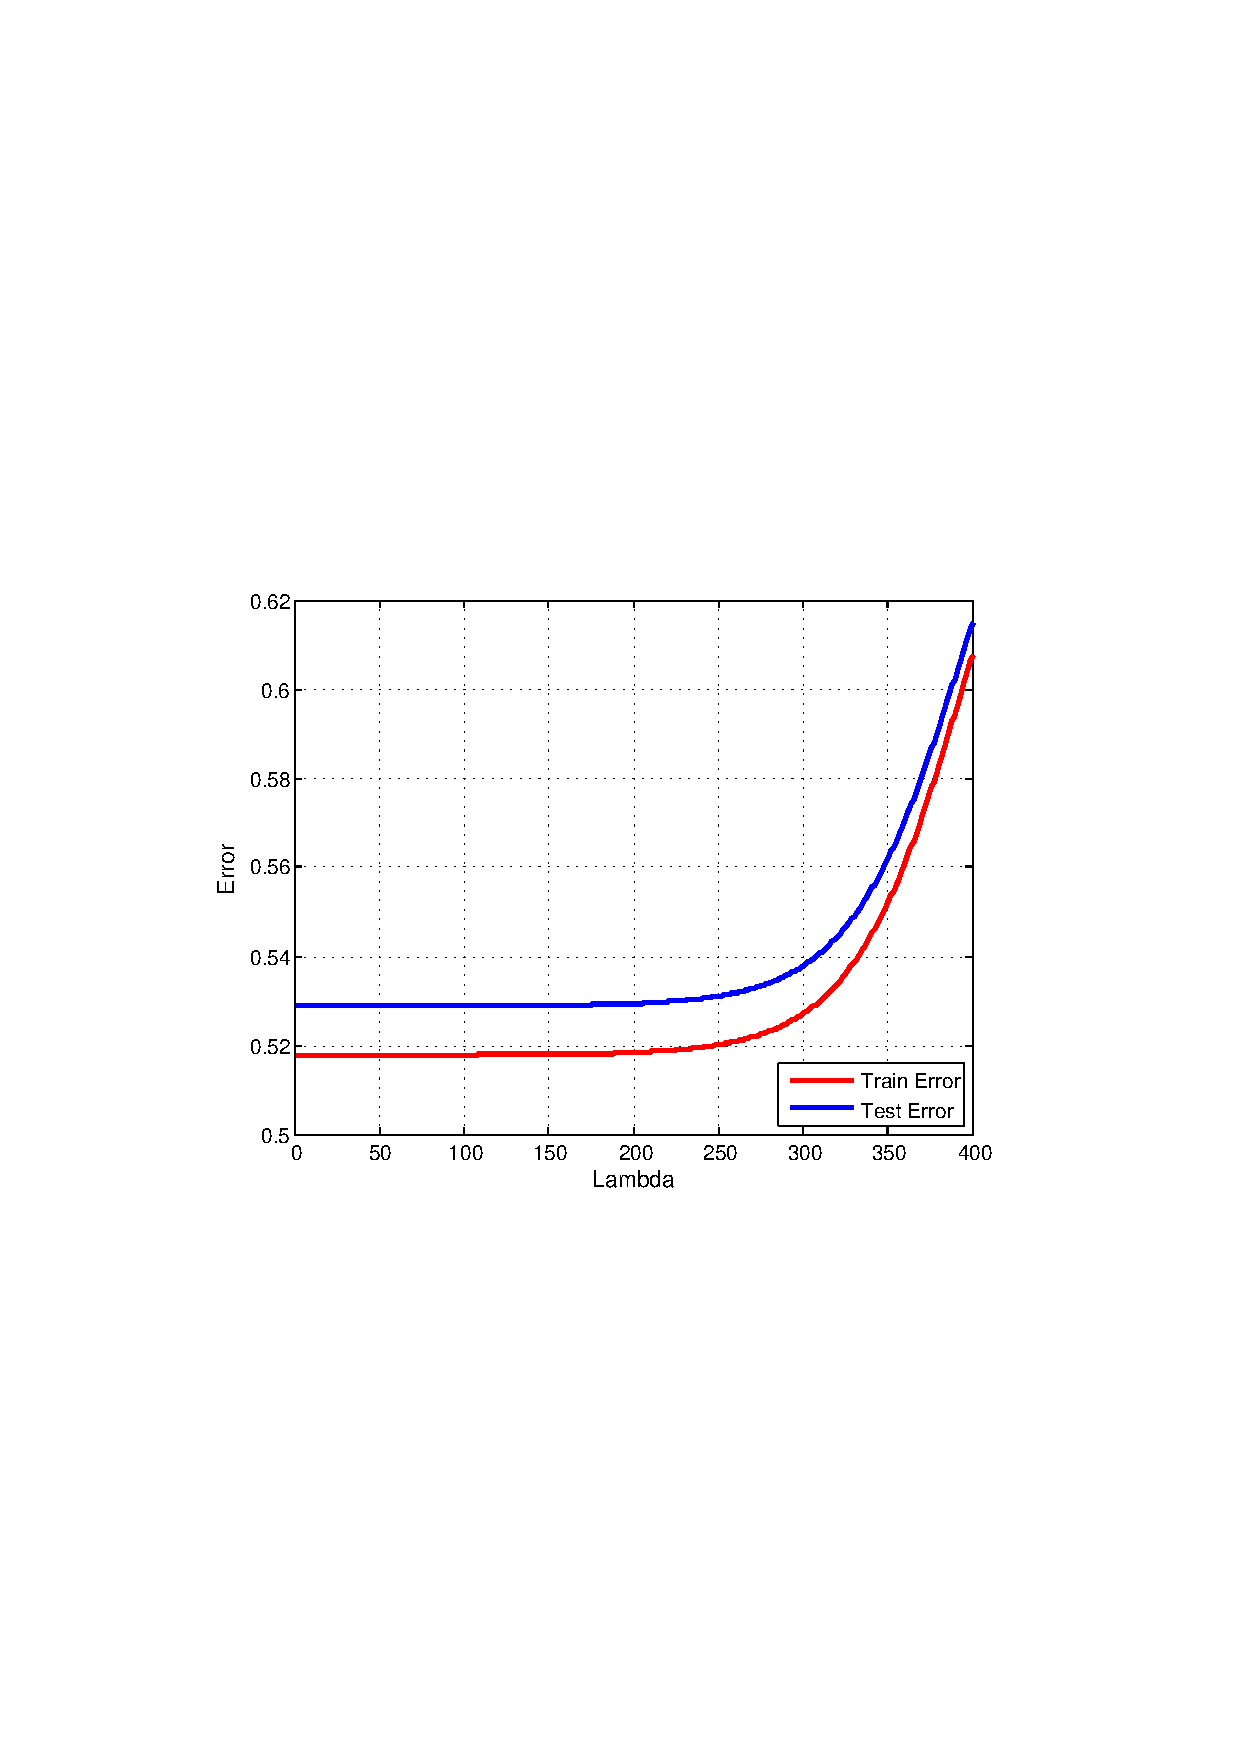
\includegraphics[clip, trim=4cm 9cm 3cm 10cm, width=\textwidth]{figures/Lambda_pLG.pdf}
    \caption{Train and test error assessment with penalty factor ($\lambda$) for penalized logistic regression
    for 50-50 split.}
    \label{fig:Lambda_pLr}
  \end{subfigure}
  \hfill
  \begin{subfigure}[b]{0.45\textwidth}
    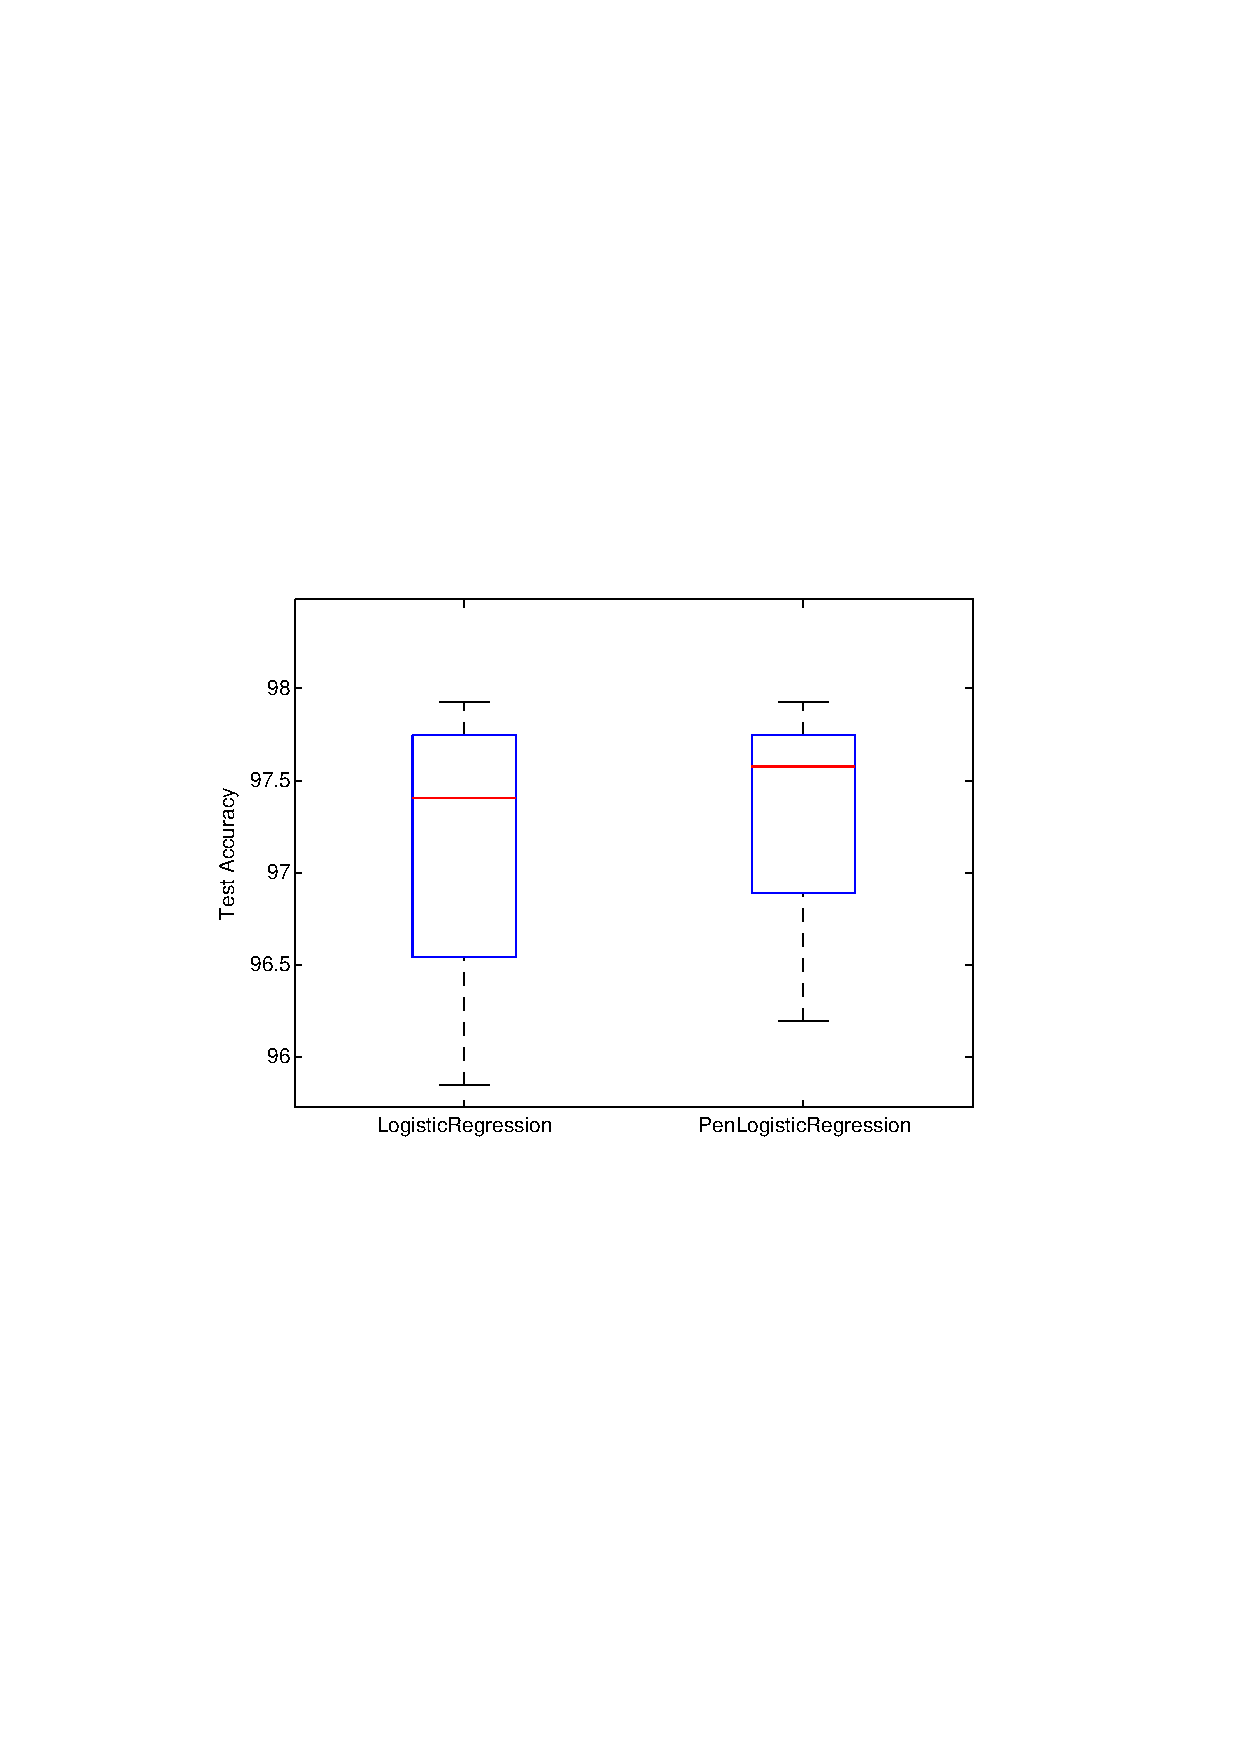
\includegraphics[clip, trim=4cm 10cm 3cm 10cm, width=\textwidth]{figures/comparison_LR_pLR.pdf}
    \caption{Comparison of logistic regression and penalized logistic regression based on validation accuracy}
    \label{fig:comp_LR_pLR}
  \end{subfigure}
\end{figure}

Best results are obtained on the test accuracy of $97.318\%$ with the values 0.1 for ($\lambda$) and 10.0 for ($\alpha$).
\ref{fig:comp_LR_pLR} shows the comparison of the logistic regression and penalized logistic regression based on the classification accuracy percentage over the test data. The improvements that is captured with the penalized logistic regression is little but significant.  

\begin{table}[h!]
\begin{center}
    \begin{tabular}{ | l | l | l | p{5cm} |}
    \hline
    Method & RMSE & 0-1-Loss & Log-Loss \\ \hline
    Logistic Regression & 0.147896 & 0.020743 & 105.151844 \\ \hline
    Pen Logistic Regression & 0.122288 & 0.014693 & 75.380959 \\ \hline
    \end{tabular}
\end{center}
\caption{Some prediction error estimates for the test data}
\label{table:test_errors}
\end{table}
 
The table \ref{table:test_errors} shows error measurements of the test data with $\alpha=10.0$ and $\lambda=1.0$ using $RMSE$, $0-1 loss$ and $log-loss$. Increasing the value of $\alpha$ decreases all error estimations until a maximum $\lambda=10.0$ value and we obtained the best prediction accuracy with this value for the $\lambda$.

\subsection{Feature transformation}
We experimented with polynomial, exponential, sqrt(abs*)) of the values
but did not manage to improve the previous results obtained using penalized logistic regression. Our best model setup (alpha = lambda = degree =) had a recognition rate of approx 96$\%$, when we used a polynomial of degree 2.
Since the model worked  and but not better just as it is
and since simpler models are preferred, we considered this not to be so relevant.